\documentclass[onecolumn,english,aps,pra]{revtex4}
\usepackage{amssymb}
\usepackage{amsmath}
\usepackage{graphicx}
\usepackage{epstopdf}
\usepackage{bm}
\usepackage{braket, float}
\usepackage{color}
\usepackage{rotating,booktabs}
\usepackage{array}
\usepackage{physics,hyperref}
\hypersetup{
    colorlinks=true,
    linkcolor=blue,
    filecolor=blue,      
    urlcolor=blue,
    citecolor=blue,
}
%\usepackage{breqn}


\begin{document}

\title{Strongly Interacting Spinors in One-Dimensional Harmonic Trap}

\maketitle

\section{General Formulation}

First we will consider two strongly-interacting, ultracold bosons with a spin degree of freedom confined in a one-dimensional harmonic trap. For now, we assume that the interaction is a spin-independent point interaction. The Hamiltonian is given by

\begin{equation}
    H = \sum_{i = 1}^{N} \left[ -\frac{1}{2} \pdv[2]{}{x} + \frac{1}{2} x_i^2 \right]
            + g \sum_{i < j} \delta(x_i - x_j)
	\end{equation}
%
where $N$ is the number of particles, the constant $g$ is the interaction strength, and we have set $\hbar = m = \omega = 1$. For spinless bosons, the many-body wave function can be found using the Bose-Fermi mapping \cite{girardeau1960relationship} in the case of $g \rightarrow \infty$.

For the case of spinful particles, Yang et al. \cite{yang2015strongly} obtain a second-order, effective Hamiltonian, which is written as
%
\begin{equation}
H_{\text{eff}} = -\frac{1}{g} \sum_{i = 1}^{N - 1}C_i(1 \pm \mathcal{E}_{i, i+1})
\label{spinchain}
\end{equation}
%
where $\mathcal{E}_{i, i+1}$ is the exchange operator that exchanges the $i^{th}$ particle with the $(i + 1)^{th}$ particle. Plus is for bosons and minus is for fermions. Each $C_i$ is a constant 
%
\begin{equation}
C_i = N \int \prod_j dx_j \left| \pdv{\varphi_A}{x_i} \right|^2 \delta(x_{i + 1} - x_{i}) \theta^1_{[i+1, i]}
\end{equation}
%
where $\varphi_F$ is the slater determinant for our system of particles, and $\theta^1_{[i+1, i]}$ is the reduced sector function given by
%
\[ \theta^1_{[i+1, i]} = \theta^1 / \theta(x_{i + 1} - x_i) 
= \frac{\theta(x_2 - x_1) \cdots \theta(x_N - x_{N-1})}{\theta(x_{i + 1} - x_i)} \]

Additionally, Yang et al. show that the one-body density matrix for these spinors can be separated into its spatial and spin components

\begin{equation}
\rho_{\sigma, \sigma'}(x, x') = \sum_{m, n} \rho_{m, n}(x, x') S_{m, n}(\sigma, \sigma')
\end{equation}
%
where the spatial component 
%
\begin{equation}
\rho_{m, n}(x', x) = (\pm 1)^{m-n} (N - 1)! \int dx_{2} \cdots dx_{N} \varphi_{A}^{*} \varphi_{A}' \theta^{(1,\ldots,m)} \theta'{}^{(1,\ldots, n)}
\end{equation}
%
is just the one-body density matrix for the sector $x_2 < x_3 < \cdots < x_m < x' \cdots x_n < x \cdots < x_N$ for $m < n$. If the particles are bosons, the $\pm$ is a minus and if fermions it is a plus. The function $\theta^{(1,\ldots, n)}$ refers to a cyclic shift backwards for the first $n$ indices of the sector function $\theta^1$, i.e., 
%
\[ \theta^{(1,\ldots, n)}(x, x_2, \ldots, x_N) = \theta^1(x_2, x_3, \ldots, x_n, x, \ldots, x_N) \]
%
More generally, the expression $(1,\ldots, n)$ denotes a cyclic permutation on the first $n$ indices
\[ x_1, x_2, \ldots, x_N \longrightarrow x_2, x_3, \ldots, x_n, x_1, x_{n+1}, \ldots, x_N \]
%
And the spin component of the one-body density matrix is
%
\begin{equation}
S_{m, n}(\sigma, \sigma') = [(1, \ldots, m) c_m(\sigma)|\chi \rangle ]^\dagger [(1, \ldots, n) c_n(\sigma')|\chi \rangle ]
\end{equation}
%
where $c_m(\sigma')$ is a destruction operator for the $m^{th}$ particle with spin $\sigma'$. For instance, $c_2(\frac{1}{2})$ destroys the second particle if it has spin $\frac{1}{2}$. If it does not, then $c_2(\frac{1}{2}) \ket{\chi} = 0$.

\section{Two Spin 1/2 Bosons}

For the case of two spin-$\frac{1}{2}$ bosons, we can see that the eigenstates of the effective hamiltonian in equation \eqref{spinchain} are just the states $| \chi \rangle$ that are symmetric under particle exchange. These eigenstates are easy to find because they correspond to the four total spin states for two spin-$\frac{1}{2}$ particles. 

We will first consider the case where we have two strongly-interacting bosons with total spin state $\ket{\chi} = \ket{ S= 1,M= 1 } = \ket{\uparrow, \uparrow}$. First we calculate the spin component. It is immediately apparent that $ c_m(\sigma') \ket{\chi}$ will be zero unless $\sigma' = \uparrow$, because that is the spin of both particles. It can be shown that for any $m, n \in \{ 1, 2 \}$

\begin{equation}
S_{m, n}(\sigma, \sigma') = 
\begin{cases}
	1 & \sigma' = \sigma = \uparrow\\
	0 & \text{else}
\end{cases}
\end{equation}

and thus our one-body density matrix is
\begin{equation}
\rho_{\uparrow, \uparrow}(x, x') = 
\rho_{1, 1}(x, x') + \rho_{1, 2}(x, x')
+ \rho_{2, 1}(x, x') + \rho_{2, 2}(x, x')
\end{equation}

We therefore need only calculate the four spatial sectors for the one-body density matrix. The simplified form of the slater determinant for two particles in a harmonic oscillator is

\begin{equation}
\varphi_F(x_1, x_2) = \frac{1}{\sqrt{\pi}} e^{-\frac{1}{2} (x_1^2 + x_2^2) } (x_2 - x_1)
\end{equation}

And so for each spatial sector of the one-body density matrix we have
\begin{align*}
\rho_{1, 1}(x, x') &= \frac{1}{\pi} \int dx_2 e^{-\frac{1}{2} (x'^2 + x^{2}) } 
 e^{-x_2^2} (x_2 - x)(x_2 - x') \theta(x_2 - x) \theta(x_2 - x)\\
\rho_{1, 2}(x, x') &= \frac{1}{\pi} \int dx_2 
e^{-\frac{1}{2} (x'^2 + x^2) } e^{-x_2^2} (x_2 - x)(x' - x_2) 
\theta(x_2 - x) \theta(x' - x_2)\\
\rho_{2, 1}(x, x') &= \frac{1}{\pi} \int dx_2 
e^{-\frac{1}{2} (x'^2 + x^2) } e^{-x_2^2} (x - x_2)(x_2 - x') 
\theta(x - x_2) \theta(x_2 - x')\\
\rho_{2,2}(x, x') &= \frac{1}{\pi} \int dx_2 e^{-\frac{1}{2} (x'^2 + x^2) } 
e^{-x_2^2} (x_2 - x)(x_2 - x') \theta(x - x_2) \theta(x' - x_2)
\end{align*}

These can be combined into a single simpler integral by rewriting each of them
\begin{align*}
\rho_{1, 1}(x, x') &= \frac{1}{\pi} \int^{\infty}_{\text{max}(x, x')} dx_2 e^{-\frac{1}{2} (x'^2 + x^2) } 
 e^{-x_2^2} (x_2 - x)(x_2 - x') \\
\rho_{2,2}(x, x') &= \frac{1}{\pi} \int_{-\infty}^{\text{min}(x, x')} dx_2 e^{-\frac{1}{2} (x'^2 + x^2) } 
e^{-x_2^2} (x_2 - x)(x_2 - x') 
\end{align*}
And we can write the sum of the other two as
\begin{align*}
\rho_{1, 2}(x, x') + \rho_{2, 1}(x, x') & = \frac{1}{\pi} \epsilon(x' - x) \int_{x}^{x'} dx_2 
e^{-\frac{1}{2} (x'^2 + x^2) } e^{-x_2^2}(x - x_2)(x_2 - x')\\
& =  \frac{1}{\pi} \int_{\text{min}(x, x')}^{\text{max}(x, x')} dx_2 
e^{-\frac{1}{2} (x'^2 + x^2) } e^{-x_2^2} (x - x_2)(x_2 - x')
\end{align*}
We can turn the sum of these terms into a single integral by noting that for each integral, the integrand is always positive, thus
%
\begin{equation}
\rho_{\uparrow, \uparrow}(x, x')
 = \frac{1}{\pi} \int dx_2 e^{-\frac{1}{2} (x'^2 + x^2) } e^{-x_2^2} |x_2 - x||x_2 - x'|
\end{equation}
%
Which is the same one-body density matrix for two spinless, hard-core bosons. Thus we should expect results for the previous case to hold regarding the Tan Contact, the Tan Contact time dependence, and Dynamical Fermionization. 

Now let's consider a slightly more interesting scenario where
$\ket{\chi} = \ket{1, 0} = 
\frac{1}{\sqrt{2}}(\ket{\uparrow, \downarrow} + \ket{\downarrow, \uparrow})$
Using mathematica code to calculate the spin component of the one-body density matrix, we find that for any $m, n \in \{ 1,2 \}$
%
\begin{equation}
S_{m, n}(\sigma, \sigma') = 
\begin{cases}
	\frac{1}{2} & \sigma' = \sigma = \uparrow\\
	\frac{1}{2} & \sigma' = \sigma = \downarrow \\
	0 & \text{else}
\end{cases}
\end{equation}
%
so the simplification of the integrals will be the same as in the previous case but now there will be a constant of $\frac{1}{2}$ out front 
\begin{equation}
\rho_{\uparrow, \uparrow}(x, x')
= \rho_{\downarrow,\downarrow}(x, x')
 = \frac{1}{2\pi} \int dx_2 e^{-\frac{1}{2} (x'^2 + x^2) } e^{-x_2^2} |x_2 - x||x_2 - x'|
\end{equation}
For a different result, we can consider the antisymmetric singlet state $\ket{\chi_S} = \ket{0,0} = 
\frac{1}{\sqrt{2}}(\ket{\uparrow, \downarrow} - \ket{\downarrow, \uparrow}) $. In this case, the following gives a strongly-interacting boson wave function with this spin configuration
\begin{equation}
\Psi(x_1, x_2;\sigma_1, \sigma_2) = \varphi_F(x_1, x_2) \chi_S(\sigma_1, \sigma_2)
\label{SingletState}
\end{equation}
If we recall from the spinless hard-core boson case, the Bose-Fermi mapping \cite{girardeau1960relationship} worked because the mapping function $A(x_1, \ldots, x_N)$ turned the fermion wave function $\Psi_F$ into a wave function that 1) satsified the same Hamiltonian, 2) satsified continuity conditions, 3) satisfied same boundary conditions as $\Psi_F$ (for HCB, $\Psi$ must go to zero when two particles occupy the same position), and 4) satisfied boson exchange statistics (i.e., symmetry under particle exchange). When all these conditions are satisfied, the result must be a hard-core boson solution.

Similarly, for the present case, equation (\ref{SingletState}) satisfies the same conditions, where the dual antisymmetry of the spatial and spin component make the overall wave function symmetric. Because the spatial component of this wave function matches the fermion spatial component, we expect that the momentum tail for (\ref{SingletState}) will display exponential decay like fermions.

\subsection{Non-separable Wave Function}

When the spin and spatial components of the wave function are not separable like they are in the last cases,
\begin{align}
\Psi(x_1, x_2; \sigma_1, \sigma_2) &= \frac{1}{\sqrt{2}}\left[\varphi_F(x_1, x_2) \chi_S(\sigma_1, \sigma_2) + \varphi_B(x_1,x_2) \chi_T(\sigma_1, \sigma_2)\right]
\label{MixedState}\\
\ket{\chi_S}& = \frac{1}{\sqrt{2}}(\ket{\uparrow, \downarrow} - \ket{\downarrow, \uparrow})\nonumber\\
\ket{\chi_T} &= \frac{1}{\sqrt{2}}(\ket{\uparrow, \downarrow} + \ket{\downarrow, \uparrow})\nonumber
\end{align}
where $\varphi_B = |\varphi_F|$, we can calculate directly from 
%
\begin{align*}
\rho_{\sigma, \sigma'}(x, x')& = 
\sum_{\sigma_2, \ldots, \sigma_N} \int dx_2 \cdots dx_N
\Psi^*(x,x_2,\ldots,x_N;\sigma, \sigma_2,\ldots,\sigma_N)
\Psi(x',x_2,\ldots,x_N;\sigma', \sigma_2,\ldots,\sigma_N)
\end{align*}
%
that the Tan contact will ultimately still be the same. 
%
\begin{align}
\rho_{\sigma, \sigma'}(x, x') &= \frac{1}{2}\sum_{\sigma_2} \int dx_2 
\left[ \varphi_F \chi_S + \varphi_B \chi_T\right]
\left[ \varphi_F' \chi_S' + \varphi_B' \chi_T'\right]\nonumber\\
& = \frac{1}{2}\sum_{\sigma_2} \int dx_2 
\varphi_B\varphi_B'\chi_T\chi_T'
+ \varphi_B\varphi_F'\chi_T\chi_S'
+ \varphi_F\varphi_B'\chi_S\chi_T'
+ \varphi_F\varphi_F'\chi_S\chi_S'
\label{MixedOBDMSimp}
\end{align}
%
Each spin combination can be simplified greatly
\begin{align*}
S_{1}(\sigma, \sigma') &\equiv \sum_{\sigma_2}\chi_T(\sigma,\sigma_2)\chi_T(\sigma',\sigma_2) 
= \sum_{\sigma_2}\chi_S(\sigma,\sigma_2)\chi_S(\sigma',\sigma_2)\\
S_{2}(\sigma, \sigma') &\equiv \sum_{\sigma_2}\chi_T(\sigma,\sigma_2)\chi_S(\sigma',\sigma_2) 
= \sum_{\sigma_2}\chi_S(\sigma,\sigma_2)\chi_T(\sigma',\sigma_2)\\
S_{1}(\sigma, \sigma') & =
\begin{cases}
	\frac{1}{2} & \sigma' = \sigma = \uparrow\\
	\frac{1}{2} & \sigma' = \sigma = \downarrow \\
	0 & \text{else}
\end{cases}\\
S_{2}(\sigma, \sigma') & =
\begin{cases}
	\frac{1}{2} & \sigma' = \sigma = \uparrow\\
	-\frac{1}{2} & \sigma' = \sigma = \downarrow \\
	0 & \text{else}
\end{cases}
\end{align*}
%
For each of the four spatial terms in the OBDM ($\varphi_B\varphi_B'$, $\varphi_B\varphi_F'$, \ldots), they will have their own separate contribution to the momentum distribution. The first term will give the normal $p^{-4}$ dependence we saw previously. The last term will decay exponentially because it is just the fermi distribution, and the second and third term will also decay exponentially
\begin{align*}
\int dx dx' dx_2 e^{-ip(x'-x)}\varphi_B(x, x_2)\varphi_F(x', x_2)
& =\frac{1}{\pi^2}\int dx \int dx' \int dx_2 e^{-ip(x'-x)} e^{-\frac{1}{2}(x^2 + x'^2) } e^{-x_2^2}|x_2 - x| (x_2 - x')\\
& =\frac{1}{\pi^2}\int dx_2 e^{-x_2^2} \int dx' e^{-ipx'} e^{-x'^2/2} (x_2 - x') \int dx e^{ipx}e^{-x^2/2}|x_2 - x|\\
\lim_{p \rightarrow \infty} \int dx e^{ipx}e^{-x^2/2}|x_2 - x| &= \frac{-2 e^{-\frac{1}{2} x_2^2}}{p^2}\\
\int dx' e^{-ipx'} e^{-x'^2/2} (x_2 - x') &= \sqrt{2\pi} e^{-p^2/2} (x_2 + ip) 
\end{align*}
Because the integral with respect to $x'$ decays exponentially with respect to momentum, the term as a whole for $\varphi_B(x, x_2)\varphi_F(x', x_2)$ will not contribute to the Tan contact. The Tan contact will still, therefore, be the same as the spinless case, because the only term that contributes has the same spatial component as spinless HCB. Thus
\begin{equation}
\lim_{p \rightarrow \infty} n_{\sigma}(p) =  \frac{1}{2}\left(\frac{2}{\pi} \sqrt{\frac{2}{\pi}} \frac{1}{p^4}\right) S_{1}(\sigma, \sigma)
\label{InitTanContact}
\end{equation}

\subsection{Real Space Density Profile}

We will also calculate the time evolution of the momentum distribution after the trap has been turned off, but first lets calculate some other physical characteristics so that we will have something to compare the long-term behavior to. We first calculate the number density in position space
\begin{align}
n_{\sigma}(x) & = N \rho_{\sigma, \sigma}(x,x)\\
& = \sum_{\sigma_2} \int dx_2 
\varphi_B\varphi_B\chi_T\chi_T
+ \varphi_B\varphi_F\chi_T\chi_S
+ \varphi_F\varphi_B\chi_S\chi_T
+ \varphi_F\varphi_F\chi_S\chi_S \nonumber
\end{align}
where our particle number $N$ is 2, thus eliminating $\frac{1}{2}$. In position space, the boson and fermion solution are the same, so
\begin{align}
n_{\sigma}(x) & = \frac{1}{2}S_1(\sigma, \sigma)(n_F(x) + n_B(x)) + 2S_2(\sigma,\sigma) \int dx_2 \varphi_F(x,x_2)\varphi_B(x,x_2)\nonumber\\
&= S_1(\sigma, \sigma)n_F(x) + S_2(\sigma,\sigma) \frac{2}{\pi} \int dx_2 e^{-(x^2 + x_2^2)} (x_2 -x ) |x_2 - x| \nonumber\\
&= S_1(\sigma, \sigma)n_F(x) + S_2(\sigma,\sigma) n_C(x)
\end{align}
where $n_F(x)$ is the real space density for two spinless fermions and $n_C(x)$ is the real density profile from the bose-fermi coupled 	terms in the OBDM
\begin{align}
n_F(x) &= \frac{e^{-x^2}(1+2x^2)}{\sqrt{\pi}} \label{nfRSDP}\\
n_C(x) &= 2 \int dx_2 \varphi_F(x,x_2)\varphi_B(x,x_2)= \frac{-2x e^{-2x^2} - e^{-x^2} (1+2x^2) \erf(x)}{\pi}
\label{ncRSDP}
\end{align}

If we plot this distribution for each value of spin $\sigma$, we obtain fig. \ref{fig:PositionDist}

\begin{figure}
\includegraphics[scale=0.6]{"../Plots/RSpaceDProfileMixedSpinor"}
\caption{We plot the real space density profile for each value of spin}
\label{fig:PositionDist}
\end{figure}

\subsection{Momentum Space Density Profile}

Now we consider the density profile in momentum space before the trap has been turned off. We start with the general expression for two particles
\begin{equation}
n_{\sigma}(p) = \frac{1}{\pi} \int dx \int dx' e^{ip(x-x')} \rho_{\sigma}(x,x')
\end{equation}

Plugging in our result from equation (\ref{MixedOBDMSimp}) and simplifying some, we can express our spin OBDM as
\begin{equation}
\rho_{\sigma, \sigma'}(x,x') = \frac{1}{2}S_1(\sigma, \sigma')(\rho_B(x,x') + \rho_F(x,x')) + \frac{1}{2}S_2(\sigma, \sigma')(\int dx_2 \varphi_F(x,x_2)\varphi_B(x',x_2) + \varphi_F(x',x_2)\varphi_B(x,x_2))
\end{equation}
We are familiar with the first two components and have calculated the momentum distribution from the boson and fermion OBDM before, thus we need only worry about the latter term. We can define our coupled term momentum space density profile as 
\begin{equation}
n_C(p) = \frac{1}{2}\frac{N}{2\pi}\int dx_2  \int dx \int dx' e^{ip(x-x')}(\varphi_F(x,x_2)\varphi_B(x',x_2) + \varphi_F(x',x_2)\varphi_B(x,x_2))
\label{ncInitMom}
\end{equation}
It can be shown that this function will be identically zero using a parity argument as follows
\begin{align*}
n_C(p) & = \frac{1}{\pi}\int dx_2  \int dx \int dx' \cos(p(x-x'))\varphi_F(x,x_2)\varphi_B(x',x_2) \\
& = \frac{1}{\pi^2}\int dx_2  \int dx \int dx' \cos(p(x-x')) e^{-\frac{1}{2} (x^2 + x'^2)} e^{-x_2^2} (x_2 -x) |x_2 - x'|\\
& = \frac{1}{\pi^2} \int dx \int dx' \cos(p(x-x')) e^{-\frac{1}{2} (x^2 + x'^2)} 
(-2x e^{-\frac{1}{2}x^2 -\frac{3}{2}x'^2} - e^{-\frac{1}{2}(x^2 + x'^2)}\sqrt{\pi} (1+2xx')\erf(x'))
\end{align*}
Note that in the last expression the entire integrand picks up a negative sign under the transformation $x \rightarrow -x$ and $x' \rightarrow -x'$, so we should expect the integral over a symmetric region to be zero. Thus, the momentum space density profile simplifies to
\begin{equation}
n_{\sigma}(p) =  \frac{1}{2}S_1(\sigma, \sigma)(n_B(p) + n_F(p))
\end{equation}
a plot of this distribution is given in figure \ref{fig:InitialMomentumProfile}.
\begin{figure}
\includegraphics[scale=0.6]{"../Plots/MomentumSpaceDProfileMixedSpinor"}
\caption{Plot of momentum space density profile for (\ref{MixedState})}
\label{fig:InitialMomentumProfile}
\end{figure}

\subsection{Time Evolution of Density Profiles}

Now we turn to the long term dynamics of the momentum space density profile after the trapping potential has been turned off. To find the time evolution of this system, we use a scaling transformation \cite{zel1998quantum}. Our two particle OBDM will evolve as
%
\begin{equation}
\rho_{\sigma, \sigma'}(x, x';t) = \frac{1}{2b} e^{\frac{i\dot{b}}{2b}(x'^2 - x^2)}\left(\left(\rho_B\left(\frac{x}{b},\frac{x'}{b};0\right) + \rho_F\left(\frac{x}{b},\frac{x'}{b};0\right)\right)
 S_1 + 
 \left( \rho_C\left(\frac{x}{b},\frac{x'}{b};0\right) + x \leftrightarrow x' \right)S_2\right)
 \label{TimeDepOBDM}
\end{equation}
where our scaling function $b(t) = \sqrt{1+t^2}$ and
\[
\rho_C(x,x';0) \equiv \int dx_2 \varphi_F(x,x_2)\varphi_B(x',x_2)
\]
%
and the momentum space density profile is
%
\begin{equation}
n_\sigma(p;t) = \frac{1}{\pi} \int dx \int dx' e^{ip(x-x')} \rho_{\sigma}(x,x';t)
\end{equation}
%
Because our OBDM can be separated into OBDM for other systems we have already studied, our expression for the momentum space density profile can be decomposed as follows
%
\begin{equation}
n_\sigma(p;t) = \frac{1}{2}\left(n_B(p;t) + n_F(p;t)\right)
 S_1 + n_C(p;t)S_2
 \label{MSDF-TimeDep}
\end{equation}
where
\begin{equation}
n_C(p;t) \equiv \frac{1}{2\pi b} \int dx \int dx' e^{ip(x-x')} e^{\frac{i\dot{b}}{2b}(x'^2 - x^2)} \left(\rho_C\left(\frac{x}{b},\frac{x'}{b};0\right) + x \leftrightarrow x'\right)
\end{equation}
Switching the integration labels around, we can simplify this integral to find that 
\begin{equation}
n_C(p;t) \equiv \frac{1}{\pi b} \int dx \int dx' \cos(p(x-x') + \frac{\dot{b}}{2b}(x'^2 - x^2))
\rho_C\left(\frac{x}{b},\frac{x'}{b};0\right)
\end{equation}
Notice that under the transformation $x\rightarrow -x$ and $x' \rightarrow -x'$, the integrand does not change sign due to the $(x'^2 -x^2)$ term. The integrand is no longer odd, so we cannot use a parity argument like we did in equation (\ref{ncInitMom}) to show the integral vanishes. In fact, the integral will be non-zero. 

Separating the momentum density profiles in equation (\ref{MSDF-TimeDep}) makes it  easier to find the $t \rightarrow \infty$ behavior because it has already been shown \cite{minguzzi2005exact} that
\begin{equation}
\lim_{t \rightarrow \infty} n_B(p;t) = n_F(p) = \frac{e^{-p^2}(1+2p^2)}{\sqrt{\pi}}
\end{equation}
and the fermi distribution does not change when the trap is turned off. Thus, we only need to find the large $t$ behavior of $n_C(p;t)$. We can simplify the expression for $n_C(p;t)$ to obtain
\begin{align*}
\frac{1}{2\pi b} \int dx \int dx' e^{ip(x-x')} e^{\frac{i\dot{b}}{2b}(x'^2 - x^2)}
\rho_C\left(\frac{x}{b},\frac{x'}{b};0\right) 
&= \frac{b}{2\pi} \int dx_2 \int dx \int dx' e^{ibp(x-x')} e^{\frac{i\dot{b}b}{2}(x'^2 - x^2)}
\varphi_F(x,x_2)\varphi_B(x',x_2)\\
&= \frac{b}{2\pi^2} \int dx_2 \int dx \int dx' e^{ibp(x-x')} e^{\frac{i\dot{b}b}{2}(x'^2 - x^2)}
e^{-\frac{1}{2}(x^2 + x'^2)}e^{-x_2^2} (x_2 -x)|x_2 - x'|
\end{align*}
Then, using the stationary phase approximation we find that
\begin{equation}
\lim_{t \rightarrow \infty} n_C(p;t) = \frac{-2pe^{-2p^2} - e^{-p^2}(1+2p^2)\sqrt{\pi}\erf(p)}{\pi}  
\label{ncMSDP-DF}
\end{equation}
which is the same function as the real space density profile from equation (\ref{ncRSDP}). In conclusion, the large $t$ behavior is therefore
\begin{equation}
\lim_{t \rightarrow \infty} n_\sigma(p;t) = S_1(\sigma, \sigma)n_F(p) + S_2(\sigma,\sigma) \frac{-2pe^{-2p^2} - e^{-p^2}(1+2p^2)\sqrt{\pi}\erf(p)}{\pi}
\end{equation} 
This result has been plotted in figure \ref{fig:nsRSDP-DF}, thus obtaining the same profile as we observed in the real space density profile prior to expansion. Additionally, in figure \ref{fig:ncRSDP-DF} we plot the time evolution of $n_C(p;t)$ during this dynamical fermionization process.\\

\begin{figure}[H]
\center
\includegraphics[scale=0.6]{"../Plots/MomentumSpaceDProfileMixedSpinorDF"}
\caption{Here is a plot of the momentum space density profile after the trap has been turned off and $t \rightarrow \infty$}
\label{fig:nsRSDP-DF}
\end{figure}

Notice that after the trapping potential has been turned off, the $\sigma = \frac{1}{2}$ particle has a predominantly negative momentum, whereas the $\sigma = -\frac{1}{2}$ particle tends to have a positive momentum. If this is the case, we should expect to see in the RSDP for both these particles that the $\sigma = \frac{1}{2}$ particle moves to the left and the $\sigma = -\frac{1}{2}$ moves to the right. Let's calculate this to check our result.

The time dependent RSDP is given by 
\begin{equation}
n_{\sigma}(x;t) = N \rho_{\sigma, \sigma}(x,x;t)
\end{equation}
and using equation (\ref{TimeDepOBDM}), we obtain the expression
\begin{equation}
n_{\sigma}(x;t) = \frac{1}{b}\left(S_1 n_F\left(\frac{x}{b};0\right) + S_2 n_C \left(\frac{x}{b}; 0\right) \right)
\end{equation}
and these two functions are given analytically in equations (\ref{nfRSDP}) and (\ref{ncRSDP}) respectively. We have created an \href{https://github.com/TimSkaras/UltraColdAtoms/blob/master/Plots/TimeEvolutionNS-RSDP.gif}{animation} of the time evolution of this RSDP.

This animation confirms that the two particles will move away from each other. We can plot the location of the two modes in the RSDP (one mode for the density profile of each $\sigma$) as a function of time to illustrate this more clearly (fig. \ref{DensityPeaks}). As a confirmation of these results, we should see that the derivative of the position curve for each of these density peaks, should approach the final momentum of each particle after dynamical fermionization has occurred. Because the final MSDP is the same distribution as the initial RSDP however, this just means that the intial value of each density peak should approximately equal the steady state slope of each density peak trajectory.

In other words, if we denote $Q_\sigma(t)$ as the location of the RSDP mode for the particle with spin $\sigma$, then our previous analysis translates to the statement
\[ Q_\sigma(0) = \lim_{t \rightarrow \infty} Q'_{\sigma}(t) \]
Numerical calculations confirm this with $Q_\sigma(0) \approx .771242$ and the best fit line for $Q_\sigma(t)$ in interval $t \in [100,150]$ has slope $m = 0.771217$. This calculation is a nice indirect result of the dynamical fermionization already discussed.

\begin{figure}[H]
\center	
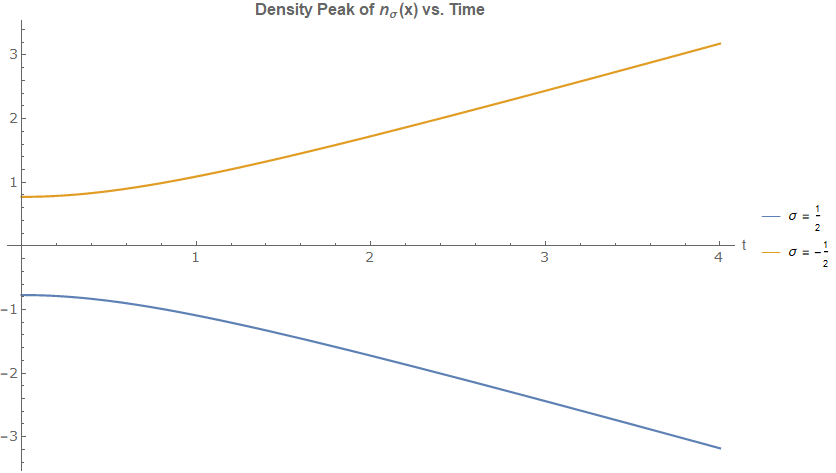
\includegraphics[scale=0.45]{../Plots/DensityPeaks}
\caption{This is a plot of the time evolution of the two modes in $n_\sigma(x)$ for each $\sigma$ after the trapping potential has been turned off. The two peaks move away from each other and approach a constant momentum.}
\label{DensityPeaks}
\end{figure}

\subsection{Non-separable Wave Function with Constant Phase Difference}

Now we consider how the above results would change if we modified equation (\ref{MixedState}) so that the two terms differed by a constant phase, viz.
\begin{equation}
\Psi(x_1, x_2; \sigma_1, \sigma_2) = \frac{1}{\sqrt{2}}\left[\varphi_F(x_1, x_2) \chi_S(\sigma_1, \sigma_2) + e^{i\theta	}\varphi_B(x_1,x_2) \chi_T(\sigma_1, \sigma_2)\right], \qquad \theta \in [0,2\pi)
\end{equation}
%
For the real space density profile (RSDP), we obtain a different expression from before
\[
n_{\sigma}^\theta(x) = \frac{1}{2}S_1(\sigma, \sigma)(n_F(x) + n_B(x)) +   S_2(\sigma,\sigma) \int dx_2 
\left[ \varphi_F(x,x_2)\varphi_B(x,x_2) e^{i\theta} + \varphi_F(x,x_2)\varphi_B(x,x_2) e^{-i\theta} \right]
\]
and we can simplify this latter term
\begin{align*}
n_C^\theta(x) & =  \int dx_2 
\left[ \varphi_F(x,x_2)\varphi_B(x,x_2) e^{i\theta} + \varphi_F(x,x_2)\varphi_B(x,x_2) e^{-i\theta} \right]\\
& = 2 \cos (\theta) \int dx_2 \varphi_F(x,x_2)\varphi_B(x,x_2)\\
& = \frac{2 \cos (\theta)}{\pi} \int dx_2 e^{-\frac{1}{2}(x^2 + x'^2)} e^{-x_2^2} (x_2 -x) |x_2 - x|\\
& = -\frac{\cos (\theta)}{\pi} (2xe^{-2x^2} + e^{-x^2}\sqrt{\pi} (1 + 2 x^2) \erf(x)) 
\end{align*}

\begin{figure}[h] 
\includegraphics[scale=0.45]{"../Plots/TimeEvolutionNC"}
\caption{Plot of the time evolution of $n_{C}(p;t)$. The splitting that occurs during dynamical fermionization of the momentum distribution for each value of spin $\sigma$ is due to the change $n_C$. The red, dashed line is the asymptotic analytic expression given in equation (\ref{ncMSDP-DF}). There is also an animated \href{https://github.com/TimSkaras/UltraColdAtoms/blob/master/Plots/TimeEvolutionNC.gif}{gif} of this time evolution.}
\label{fig:ncRSDP-DF}
\end{figure}
and thus 
\begin{equation}
n_C^\theta(x) = -\frac{\cos (\theta)}{\pi} (2xe^{-2x^2} + e^{-x^2}\sqrt{\pi} (1 + 2 x^2) \erf(x))
\end{equation}
which is the same expression for RSDP as in equation (\ref{ncRSDP}), differing only by a factor of $\cos(\theta)$ in front. We conclude that the RSDP for this new wave function is 
\begin{equation}
n_{\sigma}^\theta(x) = S_1(\sigma, \sigma)n_F(x) +  S_2(\sigma,\sigma) n_C^\theta(x)
\end{equation}
See this \href{https://github.com/TimSkaras/UltraColdAtoms/blob/master/Plots/ThetaEvolutionRSDP.gif}{gif} to observe how the $\theta$ dependence affects the RSDP. As we saw in figure \ref{fig:PositionDist}, the RSDP for  $\sigma = \frac{1}{2}$ is skewed toward negative momentum and the RSDP for  $\sigma = -\frac{1}{2}$ is skewed toward positive momentum. The gif illustrates that as we increase $\theta$ this trend is reversed once during $\theta \in [0, \pi]$ so that the $\sigma = \frac{1}{2}$ distribution is transformed into the $\sigma = -\frac{1}{2}$ distribution (and vice-versa) and then the trend is reversed once again while $\theta \in [\pi, 2\pi)$.

The momentum space density profile (MSDP) will also change with $\theta$. For the entire MSDP, we obtain the expression 
\begin{equation}
n_\sigma^\theta(p) = \frac{1}{2}\left(n_B(p) + n_F(p)\right)
 S_1 + n_C^\theta(p)S_2
\end{equation}
where $n_C^\theta(p)$ from equation (\ref{ncInitMom}) becomes
\begin{equation}
n_C^\theta(p) = \frac{1}{2}\frac{N}{2\pi}\int dx_2  \int dx \int dx' e^{ip(x-x')}(\varphi_F(x,x_2)\varphi_B(x',x_2)e^{i\theta} + \varphi_F(x',x_2)\varphi_B(x,x_2)e^{-i\theta})
\label{ncInitMomTheta}
\end{equation}
which we simplify to
\begin{align*}
n_C^\theta(p) &= \frac{1}{\pi^2}\int dx_2  \int dx \int dx' \cos(p(x-x') + \theta) e^{-\frac{1}{2} (x^2 + x'^2)} e^{-x_2^2} (x_2 -x) |x_2 - x'|\\
&= -\frac{\sin(\theta)}{\pi^2}\int dx_2  \int dx \int dx' \sin(p(x-x')) e^{-\frac{1}{2} (x^2 + x'^2)} e^{-x_2^2} (x_2 -x) |x_2 - x'|\\
\end{align*}
this integral does not have an integrand with odd parity and will have a non-zero contribution to the MSDP for $\theta \neq 0$. We have created a \href{https://github.com/TimSkaras/UltraColdAtoms/blob/master/Plots/ThetaEvolutionMSDP.gif}{gif} of how the momentum distribution changes with $\theta$. When $\theta =0$, we saw in figure \ref{fig:InitialMomentumProfile} that the momentum distribution for each spin value was symmetric with respect to $p$. As $\theta$ is increased, we see in the gif that this symmetry is broken as the distribution for each spin value is shifted toward the left or the right depending on the exact value of $\theta$ and $\sigma$.

Lastly, we consider the MSDP after the trapping potential has been turned off in the $t \rightarrow \infty$ limit. In order to calculate 
\begin{eqnarray}
n_\sigma^\theta(p;t) = \frac{1}{2}\left(n_B(p;t) + n_F(p;t)\right)
 S_1 + n_C^\theta(p;t)S_2\\
\lim_{t \rightarrow \infty} n_\sigma^\theta(p;t) = n_F(p;t)S_1 + \lim_{t \rightarrow \infty} n_C^\theta(p;t)S_2
\end{eqnarray}
we must find the limit of the last term. Starting with the inital $\theta$ dependent expression
\begin{equation}
n_C^\theta(p;t) \equiv \frac{b}{\pi^2} \int dx \int dx' \int dx_2  \cos(bp(x-x') + \frac{\dot{b}b}{2}(x'^2 - x^2) + \theta)
e^{-\frac{1}{2}(x^2 + x'^2)}e^{-x_2^2}(x_2 -x) |x_2 -x'|
\end{equation}
expanding the cosine in terms of exponentials and applying the stationary phase approximation again leaves us with the following asymptotic expression
\begin{equation}
\lim_{t\rightarrow \infty} n_C^\theta(p;t) = \frac{\cos(\theta)}{\pi}(-2pe^{-2p^2}-e^{-p^2}(1+2p^2)\sqrt{\pi}\erf(p))
\end{equation}
differing from the previous asymptotic expression when $\theta$ was excluded (\ref{ncMSDP-DF}) only by a factor of $\cos(\theta)$. The $\theta$-dependence will be the same as for the RSDP, therefore. Again, we have created a \href{https://github.com/TimSkaras/UltraColdAtoms/blob/master/Plots/ThetaEvolutionMSDP-DF.gif}{gif} to animate this $\theta$ dependence.

% Insert stuff about full MSDP time dependence for various theta
An animation of the full time dependence for various theta can be viewed \href{https://github.com/TimSkaras/UltraColdAtoms/tree/master/Plots/Time%20Evolution%20NSigma}{here}

\begin{figure}[h] 
\includegraphics[scale=0.55]{"../Plots/SpinorTanContactTimeDependence"}
\caption{This is a plot of the time dependence of the Tan Contact for $n_\sigma(p)$ with $\sigma = \frac{1}{2}$ and $\sigma = -\frac{1}{2}$. $C_+(t)$ denotes the Tan Contact for the former and $C_-(t)$ denotes the Tan Contact for the latter. To examine just the time dependent behavior, the Tan Contact function has been divided by its value at $t = 0$. The calculations required for this plot assumed that $\theta = 0$. These plots were created by numerically calculating the Tan Contact for several values of $t$ and then interpolating intermediate points for the sake of plotting.}
\label{fig:TanContactTimeDep}
\end{figure}

Inspecting equation (\ref{ncInitMomTheta}) again, we see that the $n_B$ term is the only term that contribute to the Tan Contact of $n_\sigma$ because all the other terms decay exponentially with $p$. The time dependence of the Tan Contact, therefore, will be the same as in the spinless HCB case, differing only by a constant. We have numerically calculated and plotted this time dependence in the plot in figure \ref{fig:TanContactTimeDep}. The plot shows that numerical calculation agrees with theoretical prediction that the Tan Contact should have a decay proportional to $\frac{1}{b(t)^3}$, where the constant is given in equation (\ref{InitTanContact}).

\pagebreak
\bibliographystyle{abbrv}
\bibliography{Two_Spinors}

\end{document}
